\documentclass{beamer}

\usepackage[utf8]{inputenc}
\usepackage[T1]{fontenc}
\usepackage{kantlipsum}
\usepackage{listings,xcolor}
\usepackage{inconsolata}
\usepackage{spverbatim}

\definecolor{dkgreen}{rgb}{0,.6,0}
\definecolor{dkblue}{rgb}{0,0,.6}
\definecolor{dkyellow}{cmyk}{0,0,.8,.3}

\lstset{
  language         = php,
  basicstyle       = \scriptsize\ttfamily,
  keywordstyle     = \color{dkblue},
  stringstyle      = \color{red},
  identifierstyle  = \color{dkgreen},
  commentstyle     = \color{gray},
  emph             =[1]{php},
  emphstyle        =[1]\color{black},
  emph             =[2]{if,and,or,else},
  emphstyle        =[2]\color{dkyellow}
  showstringspaces = false,
  numbers          = left,
  }

\usepackage{xstring}
\usepackage{catchfile}

\newcommand{\gitfolder}{.git}
\CatchFileDef{\headfull}{\gitfolder/HEAD}{}
\StrGobbleRight{\headfull}{1}[\head]
\StrBehind[2]{\head}{/}[\branch]
\CatchFileDef{\commit}{\gitfolder/refs/heads/\branch}{}
\StrGobbleRight{\commit}{1}[\longcommithash]

\newcommand{\gitrevisionlong}{%
	\longcommithash%
}

\newcommand{\gitrevisionsmall}{%
	\StrLeft{\longcommithash}{7}%
}


\title{Lazy collection}
\subtitle{Let your code procrastinate}
\institute{AFUP}
\date[2021]{Mai 2021}
\author[Pol]{Pol Dellaiera}
\logo{
    \vspace{-.3cm}
    \tikz{
        \node[opacity=0.15, inner sep=0.10cm, outer sep=0cm]{
            
\includegraphics[scale=0.35, keepaspectratio]{afup/style/logo/afup-icon+name-color}
        }
    }
}

\usetheme{afup}

% From https://jayrobwilliams.com/posts/2019/10/better-beamer
\makeatletter
\renewcommand{\itemize}[1][]{%
	\beamer@ifempty{#1}{}{\def\beamer@defaultospec{#1}}%
	\ifnum \@itemdepth >2\relax\@toodeep\else
	\advance\@itemdepth\@ne
	\beamer@computepref\@itemdepth% sets \beameritemnestingprefix
	\usebeamerfont{itemize/enumerate \beameritemnestingprefix body}%
	\usebeamercolor[fg]{itemize/enumerate \beameritemnestingprefix body}%
	\usebeamertemplate{itemize/enumerate \beameritemnestingprefix body begin}%
	\list
	{\usebeamertemplate{itemize \beameritemnestingprefix item}}
	{\def\makelabel##1{%
			{%
				\hss\llap{{%
						\usebeamerfont*{itemize \beameritemnestingprefix item}%
						\usebeamercolor[fg]{itemize \beameritemnestingprefix item}##1}}%
			}%
		}%
	}
	\fi%
	\setlength\itemsep{\fill}
	\ifnum \@itemdepth >1
	\vfill
	\fi%
	\beamer@cramped%
	\raggedright%
	\beamer@firstlineitemizeunskip%
}
\def\enditemize{\ifhmode\unskip\fi\endlist%
	\usebeamertemplate{itemize/enumerate \beameritemnestingprefix body end}
	\ifnum \@itemdepth >1
	\vfil
	\fi%
}
\makeatother

\usepackage{environ}

\newcommand{\sepframe}[2]{
    \setbeamercolor{background canvas}{bg=afupbluebackground}

    \begin{frame}[noframenumbering,plain]
        \begin{tikzpicture}[remember picture,overlay]
            \fill[afuppink] (0,0) rectangle(.05,\paperheight);
        \end{tikzpicture}
      \begin{tikzpicture}[remember picture,overlay]
          \ifx\insertframesubtitle\@empty%
              {\node[anchor=west, afupblue, font=\huge] at (0,.25){\uppercase\expandafter{#1}};}
          \else%
              {
                  \node[anchor= west, afupblue, font=\huge] at (0,.25){\uppercase\expandafter{#1}};%
                  \node[anchor= west, afuppink,font=\small] at (0,-.5){\uppercase\expandafter{#2}};}%
          \fi
      \end{tikzpicture}

      \begin{tikzpicture}[remember picture, overlay]
          \node at (current page.south east) {
              
\includegraphics[trim=0 -4cm -4cm 0, scale=.35, keepaspectratio]{src/afup/style/logo/afup-icon-color}
            };
      \end{tikzpicture}
    \end{frame}
  }

\NewEnviron{sepFrameA}[3][]{%
    \begin{frame}
        \begin{columns}
            \column{\paperwidth}
                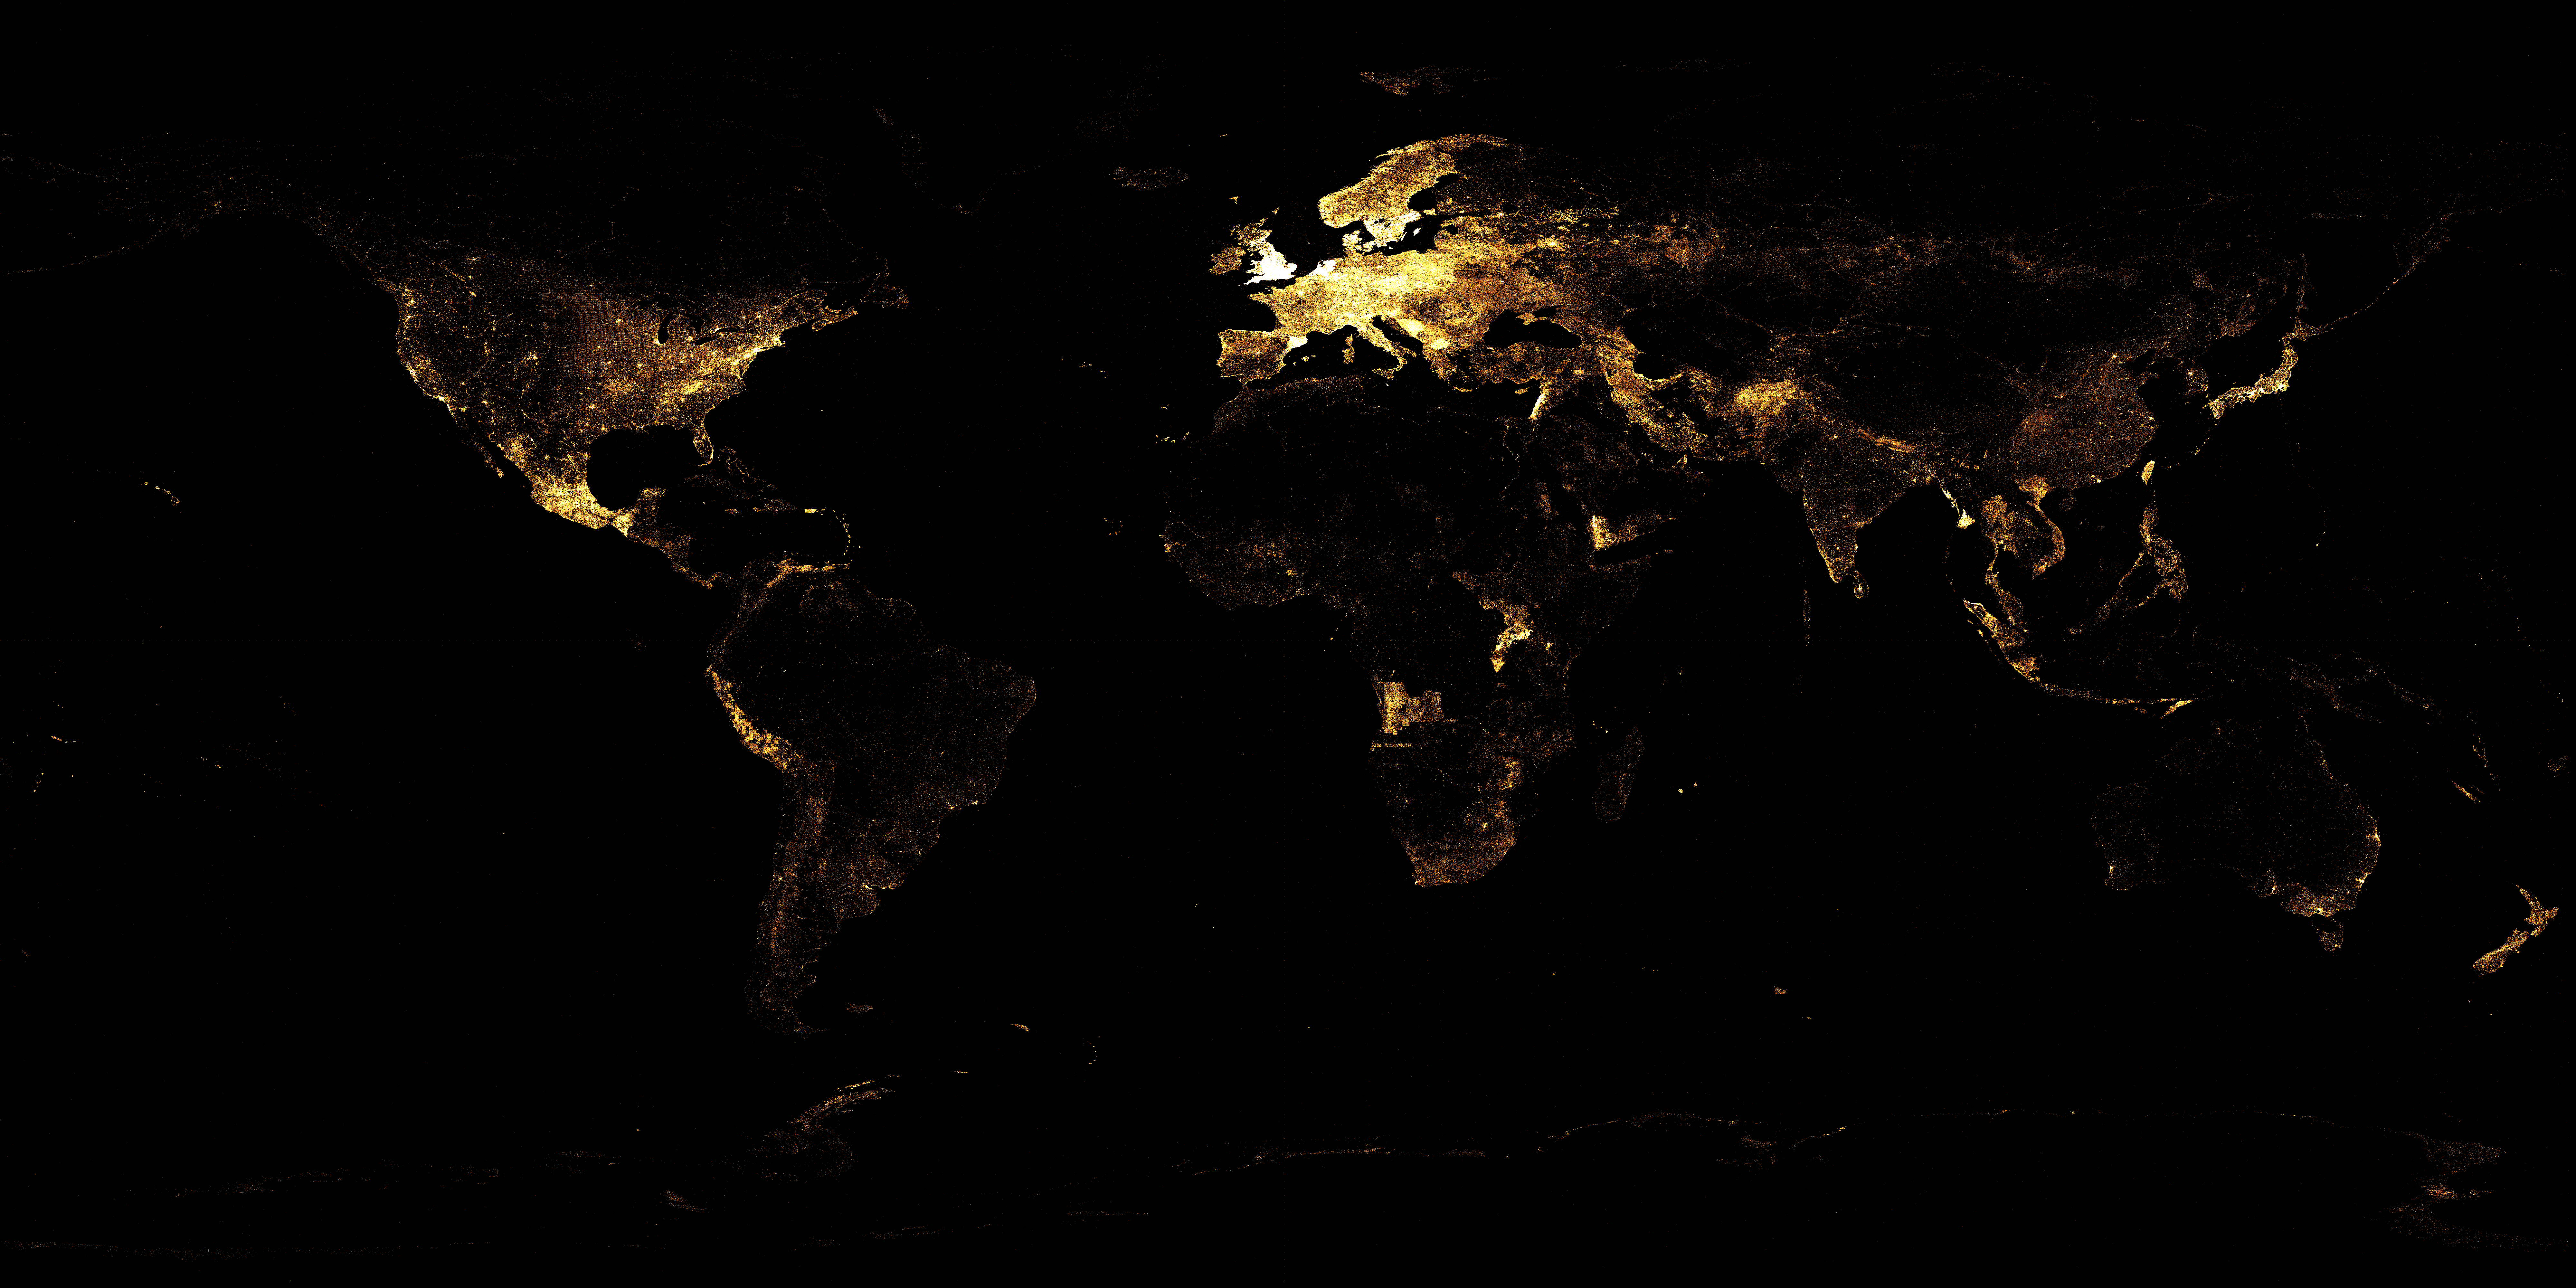
\includegraphics[width=\the\paperwidth, height=.5\paperheight]{src/afup/style/logo/bg1}
            \begin{tikzpicture}
                \node[shape=rectangle, text opacity=1,minimum height=.5\paperheight, minimum width=\paperwidth, anchor=south]{
                    \BODY
                };
            \end{tikzpicture}
          \end{columns}
    \end{frame}
}

\NewEnviron{sepFrameB}[3][]{%
    \begin{frame}
        \begin{columns}
            \column{.5\paperwidth}
                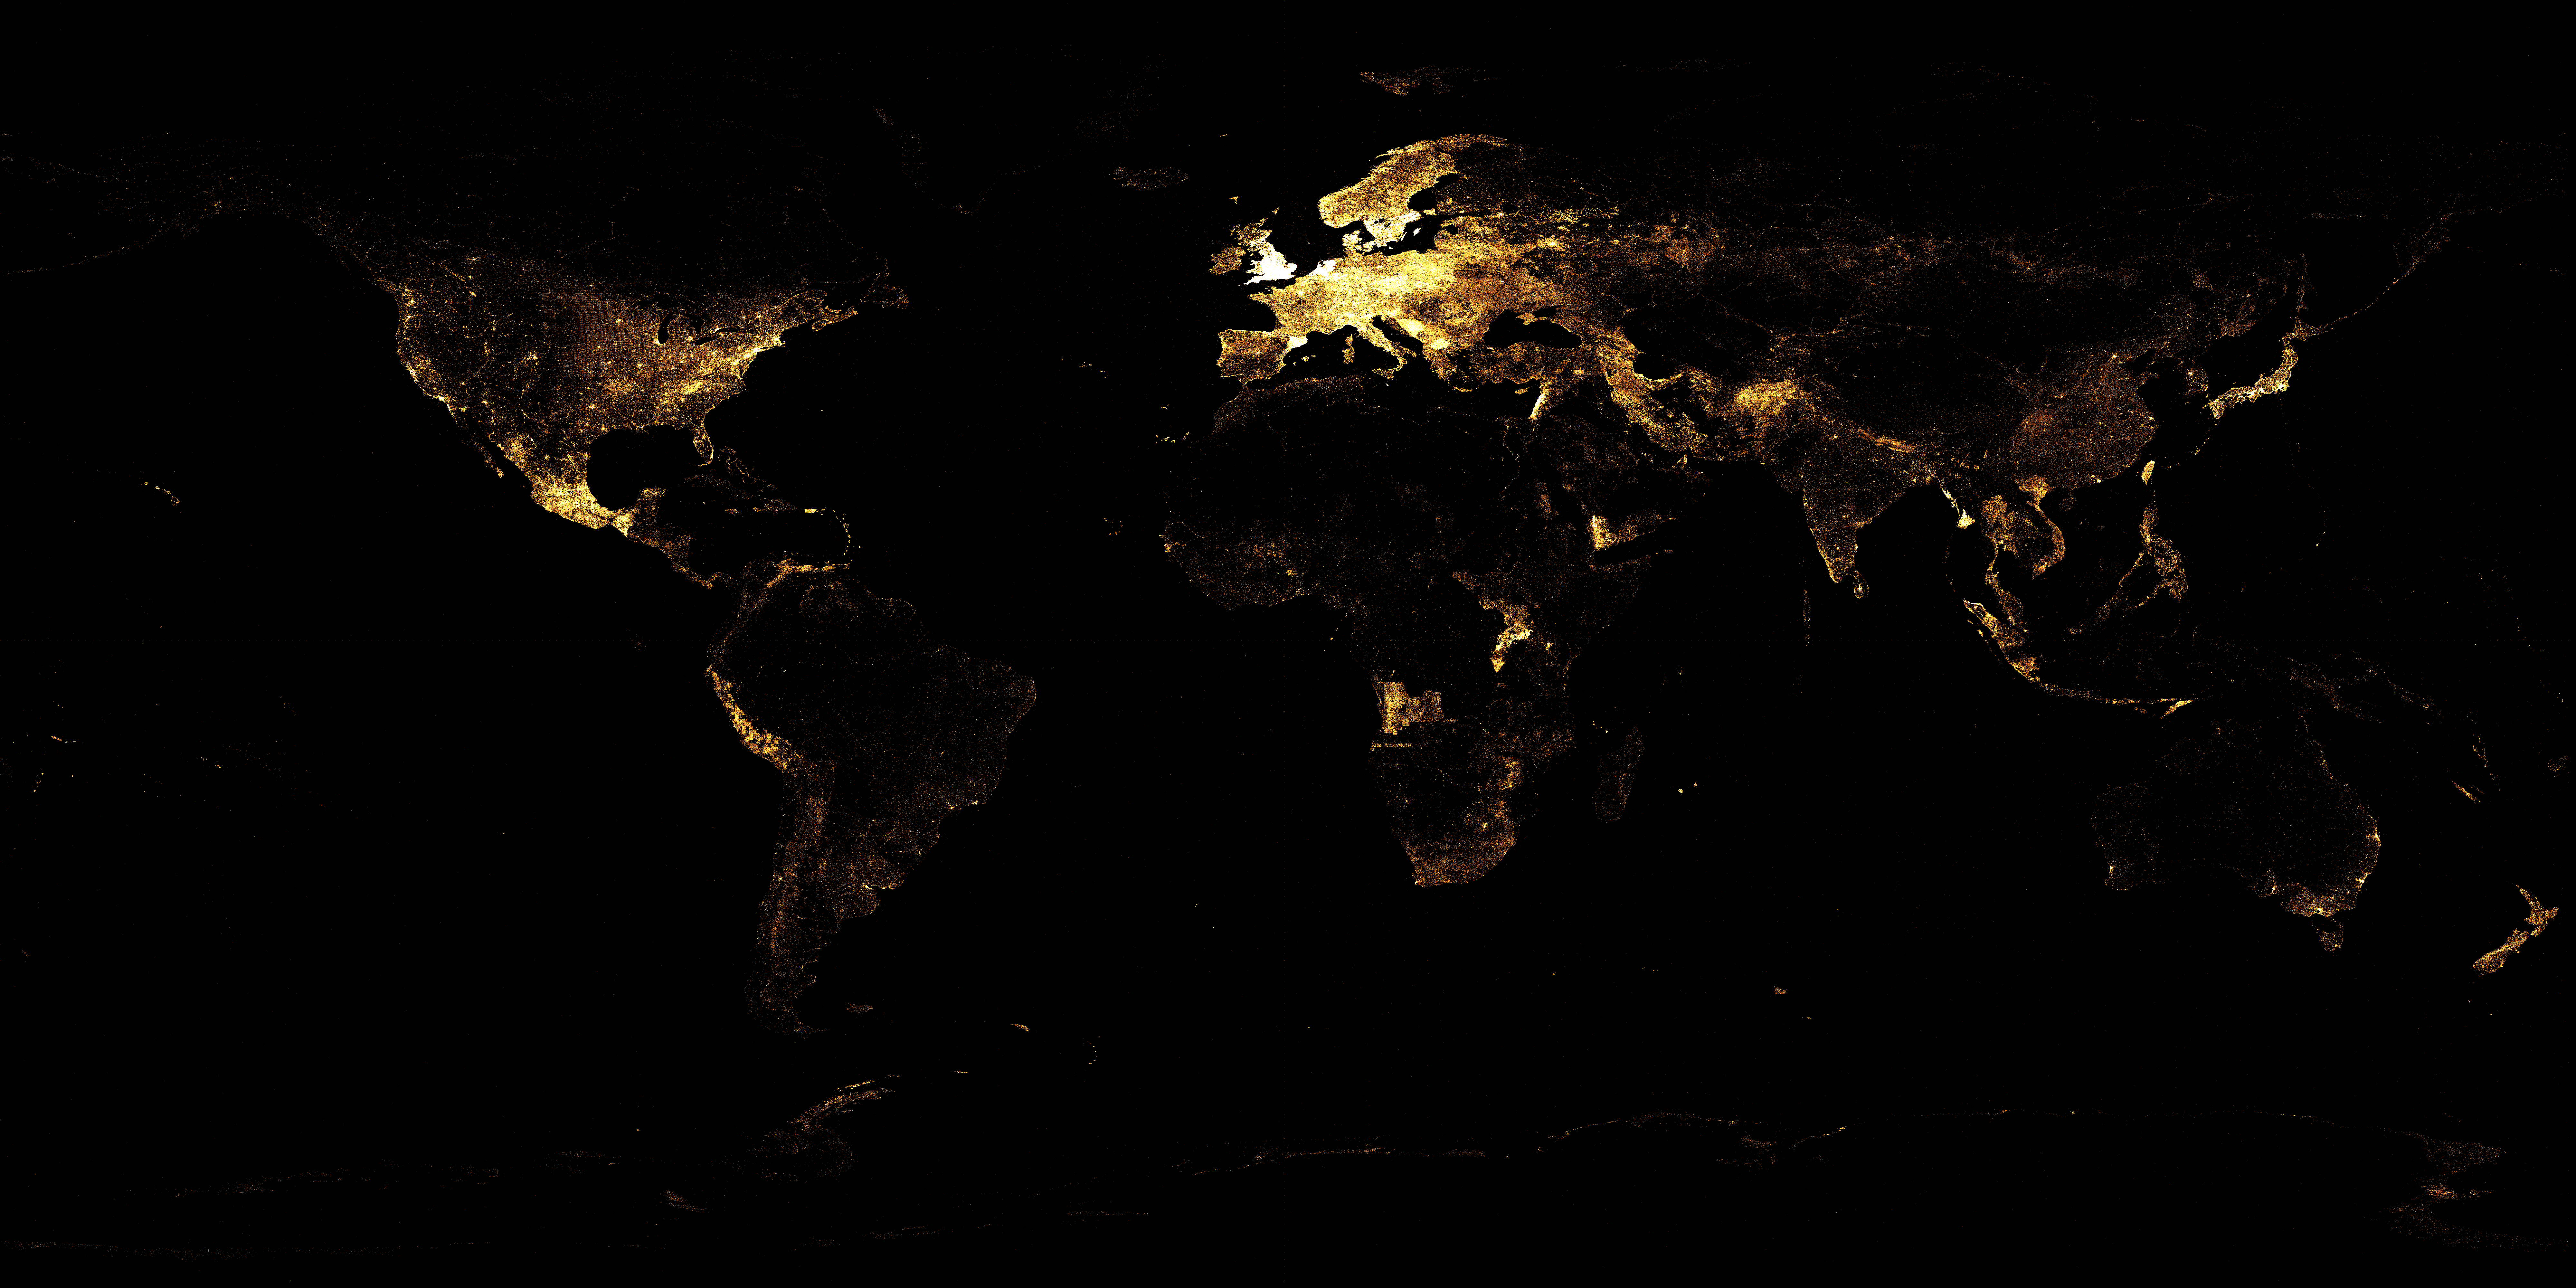
\includegraphics[width=.5\paperwidth, height=\paperheight]{src/afup/style/logo/bg1}
            \column{.5\paperwidth}
                \begin{tikzpicture}
                    \node[shape=rectangle, text opacity=1,minimum height=\paperheight, minimum width=.5\paperwidth, anchor=east]{
                        \BODY
                    };
                \end{tikzpicture}
        \end{columns}
    \end{frame}
}


% To read: https://tex.stackexchange.com/questions/113410/removing-sidebar-from-a-single-beamer-frame
% To read: https://github.com/deuslirio/UFGTeX-Presentation
% To read: https://github.com/matze/mtheme


\begin{document}

\begin{frame}[plain]
	\titlepage{}
\end{frame}

\begin{frame}[allowframebreaks]
	\frametitle{Simple frame title}
	\framesubtitle{Simple frame \textit{reductio ad absurdum}}
\end{frame}


\begin{sepframe}{Definition}{Définir une collection ?!}

\end{sepframe}

\begin{frameA}{Title}{Subtitle}
Body
\end{frameA}

\begin{frameB}{Definition}{Définir une collection ?!}
Some text here
\end{frameB}

\section{section 1}
\begin{frame}
	\frametitle{Une collection}
    \framesubtitle{Definition}

    \begin{itemize}
        \item Une collection est une structure unifiée pour représenter et manipuler un ensemble de données.
        \item Permettant de les manipuler indépendamment de ce qu'elles contiennent.
        \item Elle permettent de réduire l'effort tout en améliorant les performances\footnotemark.
        \item Favorise l'interoperabilité
        \item Favorise la réutilisation
        \item Inclus des implémentations et algorithmes pour manipuler les données
    \end{itemize}

    \footnotetext[1]{A test footnote in the first column}
\end{frame}

\begin{frame}
	\frametitle{Pourquoi}
    \framesubtitle{Fixer les \textit{incohérences}}

    PHP dispose de plusieurs structures natives propice à l'itération

    \begin{itemize}[<+->]
        \item \texttt{array}
        \item Interface \texttt{ArrayAccess}
        \item Iterateur
        \item Generateur
    \end{itemize}
\end{frame}

\begin{frame}
	\frametitle{Pourquoi}
    \framesubtitle{Fixer les \textit{incohérences}}

    PHP dispose de plusieurs fonctions natives propice à l'itération

    \begin{itemize}[<+->]
        \item \texttt{array\_map()}
        \item \texttt{array\_filter()}
        \item \texttt{array\_reduce()}
        \item \texttt{iterator\_to\_array()}
    \end{itemize}
\end{frame}

\begin{frame}
	\frametitle{Pourquoi}
    \framesubtitle{Fixer les \textit{incohérences}}

    PHP dispose de plusieurs structure indispensable pour itérer

    \begin{itemize}[<+->]
        \item \texttt{for}
        \item \texttt{foreach}
        \item \texttt{while}
    \end{itemize}
\end{frame}

\begin{frame}
	\frametitle{Incohérences}
    \framesubtitle{Array}

    \begin{itemize}[<+->]
        \item Manque de consistence (\texttt{array\_*()})
        \item Pas de vérification des types
        \item Performances
        \item Pas de gestion des erreurs
    \end{itemize}
\end{frame}

\begin{frame}
	\frametitle{Incohérences}
    \framesubtitle{PHP}

    \begin{itemize}[<+->]
        \item Manque de consistence dans les fonctions du genre \texttt{array\_*()}
        \item Les fonctions d'itérations ne fonctionnent que pour les arrays. Quid du type \texttt{iterable}?
    \end{itemize}
\end{frame}

\begin{frame}
	\frametitle{Incohérences}
    \framesubtitle{PHP}

    \begin{itemize}[<+->]
        \item \texttt{array\_map(\$callable, \$array)}
        \item \texttt{array\_map(\$array, \$callable)}
    \end{itemize}
\end{frame}

\begin{frame}
	\frametitle{Incohérences}
    \framesubtitle{PHP/array\_map()}

    Un array est composé de ...

    \begin{itemize}[<+->]
        \item clés
        \item valeurs
    \end{itemize}

    \pause

    Cependant...

    \pause

    \begin{itemize}[<+->]
        \item Signature: \texttt{array\_map(\$callable, \$array)}
        \item Callable: \texttt{\$callable(\$value)}
    \end{itemize}
\end{frame}

\begin{frame}
	\frametitle{Incohérences}
    \framesubtitle{Pourquoi?!}

    \begin{itemize}[<+->]
        \item Pourquoi un tableau est composé de 2 types de données?
        \item Pourquoi la plupart des fonctions natives ne nous permettent pas d'utiliser les 2?
    \end{itemize}
\end{frame}

\begin{frameC}{Bref...}

\end{frameC}

\begin{frame}
	\frametitle{Pourquoi}
    \framesubtitle{Fixer les \textit{incohérences}}

    \begin{quote}
        Je fais du vélo le matin, je voudrais ne pas respirer la poussière générée
        par ces datacenters fous fonctionnant si mal avec des algorithmes,
        car on se donne entre les mains un pouvoir qu'il ne maîtrise pas.

        \begin{flushright}
            \tiny{---Julien Pauli}
        \end{flushright}
    \end{quote}
\end{frame}

\begin{frame}
	\frametitle{Pourquoi}
    \framesubtitle{Fixer les \textit{incohérences}}

    \begin{quote}
        Si vous voulez être un meilleur programmeur, apprenez un autre language que
        le PHP. Si possible un language fonctionnel.

        \begin{flushright}
            \tiny{---Larry Garfield}
        \end{flushright}
    \end{quote}
\end{frame}

\end{document}
